\section{АНАЛИЗ ПОДХОДОВ К РЕШЕНИЮ ПОСТАВЛЕННОЙ ЗАДАЧИ}
\label{sec:domain}
\subsection{Анализ предметной области}
Медицина является очень важной предметной областью для человечества, так как она непосредственно связана с жизнью и здоровьем человека.Благодаря научным достижениям в области медицины люди проживают более долгую и комфортную жизнь. Знания области медицины актуальны для всех: как для врачей и студентов-медиков, так и для людей, не связанных с данной сферой. Создание интеллектуальной справочной системы поможет решить проблему структуризации большого объёма знаний в сфере
медицины. Преимуществами данной системы будут являться единство в определении терминов, а также возможность дополнения её новыми знаниями, что очень важно, учитывая то, что количество информации в сфере медицины непрерывно растёт.

В ИСС по медицине можно выделить раздел:
\begin{itemize}
	\item раздел дерматологии;
\end{itemize}

\subsection{Сравнительный анализ аналогов}

Рассмотрим несколько аналогов ИИС по медицине, а также обратим внимание на их достоинства и недостатки.

\begin{enumerate}
	\item{
		Медицинская информационная платформа \cite{medelement}
		\newline
		Достоинства:
		\begin{itemize}
			\item{Наличие полезных советов для здоровья;}
			\item{Ясность языка изложенного материала;}
			\item{Наличие справочника болезней и терминов;}
			\item{Наличие онлайн-консультаций;}
		\end{itemize}
		Недостатки:
		\begin{itemize}
			\item {Сложный интерфейс системы;}
			\item {Понятия не разделены на разделы;}\\
		\end{itemize}
		На рисунке ~\ref{fig:sections/medelement} изображен фрагмент Медицинской информационной платформы MedElement
    \begin{figure}[H]
    	\centering
    	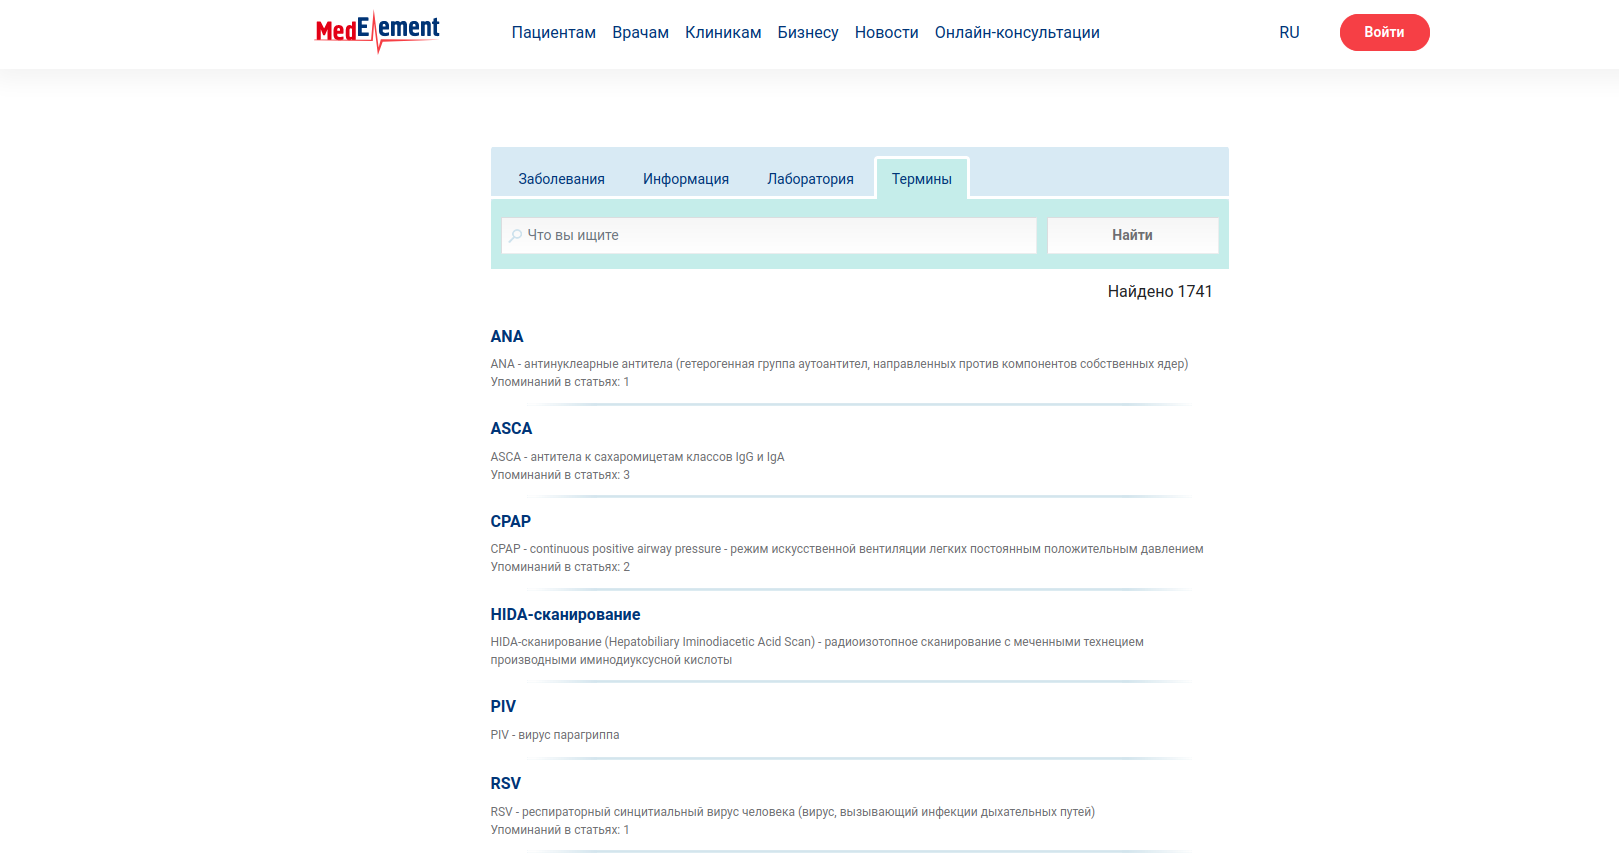
\includegraphics[width=1.0\textwidth]{sections/medelement}
    	\caption{Медицинская информационная платформа  (MedElement)}
     	\label{fig:sections/medelement}
    \end{figure} } 
	\item{
		Медицинская поисковая система \cite{medportal}
		\newline
		Достоинства:
		\begin{itemize}
			\item{Наличие перечня клиник, болезней и способов лечения;}
			\item{Разбиение всей информации на множество разделов медицины;}
			\item{Большое количество статей о здоровье;}
		\end{itemize}
		Недостатки:
		\begin{itemize}
			\item{Информация недостаточно структурирована;}
			\item {Неудобный интерфейс системы;}\\
		\end{itemize}
		На рисунке ~\ref{fig:sections/medportal} изображен фрагмент Медицинской поисковой системы МедПортал
		\begin{figure}[H]
    	\centering
    	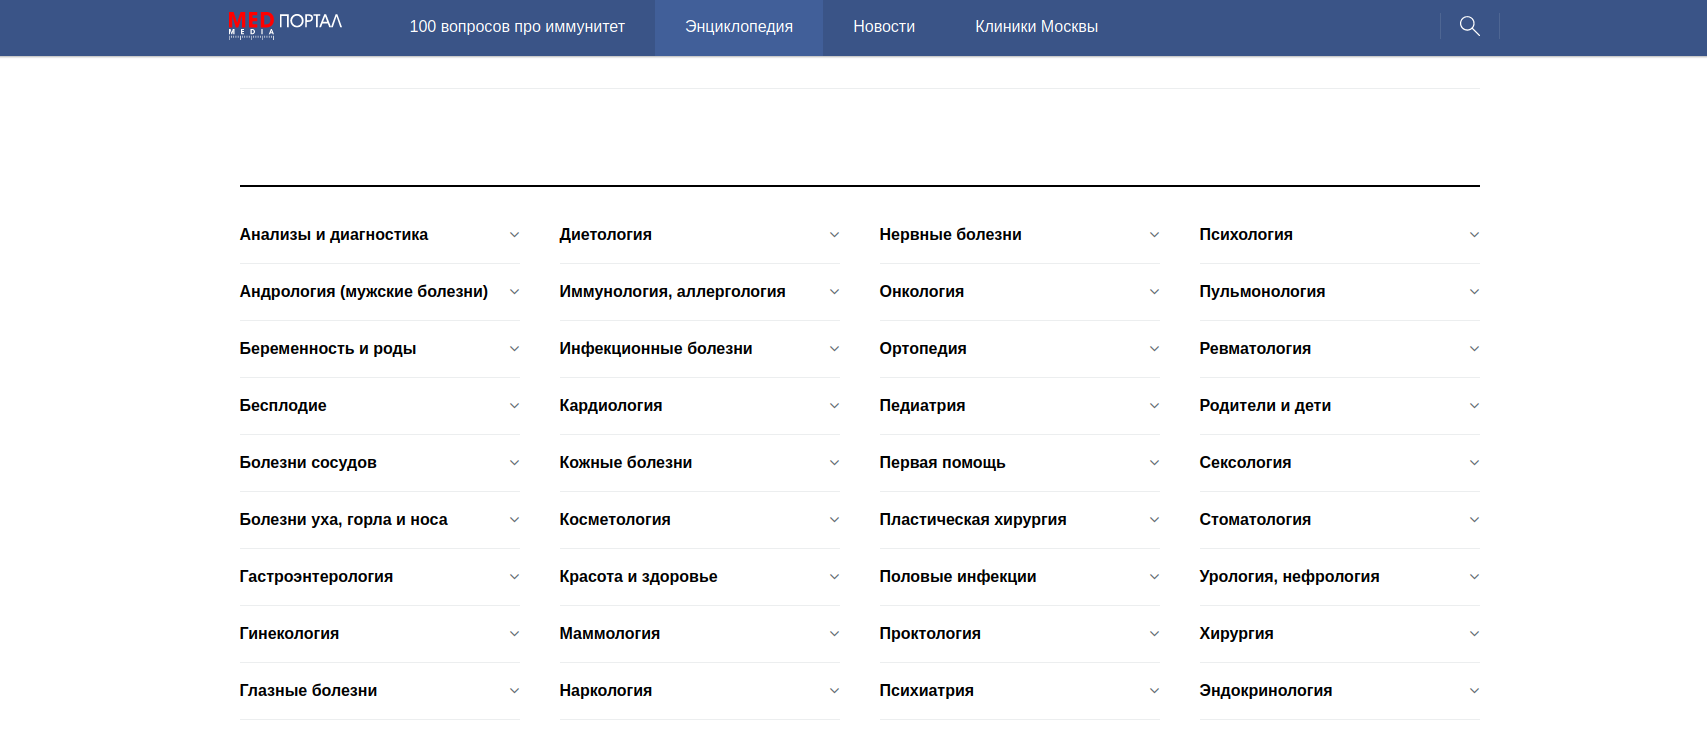
\includegraphics[width=1.0\textwidth]{sections/medportal}
    	\caption{Медицинская поисковая система (МедПортал)}
     	\label{fig:sections/medportal}
    \end{figure}}

\end{enumerate}


\subsection{Анализ подходов к разработке баз знаний}
Для разработки базы знаний может использоваться:
\begin{itemize}
    \item Технология OSTIS(Open Semantic Technology for Intelligent Systems);
\end{itemize}
OSTIS - открытая семантическая технология проектирования интеллектуальных систем. OSTIS позволяет представить знания в виде семантических сетей, посредством использования SC-кода (Semantic Computer Code).
 
Основные положения:
\begin{itemize}
	\item база знаний OSTIS может описывать любой вид знаний; 
	\item решатель задач OSTIS основан на многоагентном подходе и позволяет легко комбинировать любые модели решения задач;
	\item интерфейс ostis-системы представляет собой подсистему со своей БЗ и решателем задач (также может быть описан с помощью SC-кода);
	\item использование универсального способа представления (кодирования) информации, получившего название SC-код.\cite{OSTIS}
\end{itemize}

Достоинства:
\begin{itemize}
	\item унифицированность представления (любая информация представляется одинаково);
	\item любые знания и модели решения задач легко интегрируются в ostis-систему и её всегда можно переобучить;
	\item ostis-система может включать в себя компоненты, разработанные на базе OSTIS, а также объединяться с любыми другими системами и интегрировать другие компоненты через специальный протокол обмена информацией (JSON) и/или программный интерфейс (API);
	\item производительность ostis-системы не хуже традиционной системы, а иногда может оказаться лучше за счёт параллельной обработки (при переходе на семантические компьютеры производительность будет ещё выше).
\end{itemize}

Алфавит SC-кода представляет собой базовое синтаксическое разбиение множества sc-элементов на следующие виды (синтаксически задаваемые классы):
\begin{itemize}
	\item sc-узел;
	\item sc-ребро;
	\item sc-дуга общего вида;
	\item sc-дуга основного вида;
\end{itemize}

SC-код позволяет представлять знания в унифицированном виде.\\

\begin{itemize}
	\item Semantic Web;
\end{itemize}

Семантическая паутина — надстройка над существующей Всемирной паутиной, придуманная для того, чтобы сделать размещаемую в Интернете информацию пригодной для машинной обработки. Доступная в сети информация удобна для прочтения человеком. Семантическая паутина создана для того, чтобы сделать информацию пригодной для автоматического анализа, синтеза выводов и преобразования как самих данных, так и сделанных на их основе заключений в различные представления, полезные на практике. 

Достоинства:
\begin{itemize}
	\item большая доступность данных;
	\item облегченный поиск информации и её объединение;
	\item расширенные возможности машинной обработки предметных областей. Semantic Web-технология позволяет создавать семантические модели для предметных областей, что открывает возможности для автоматической обработки источников данных, автоматической генерации комментариев, анализа данных;
	\item улучшенная межбазовая интеграция. Semantic Web позволяет интегрировать данные из различных источников в некой мере автоматически, что ведет к экономии времени и ресурсов для создания новых баз данных либо настройки уже существующих. 
\end{itemize}

Машинная обработка возможна благодаря двум характеристикам семантической паутины:
\begin{itemize}
	\item наличие URI;
	\item использование семантических сетей и онтологий. 
\end{itemize}

URI — унифицированный идентификатор ресурса или адрес, используемый для указания ссылок на какой-либо объект (например, веб-страницу, файл или ящик электронной почты). URI используются для именования объектов. Каждый объект глобальной семантической сети имеет уникальный URI. URI однозначно называет некоторый объект. Отдельные URI создают не только для страниц, но и для объектов реального мира (людей, городов, художественных произведений и так далее), и даже для абстрактных понятий (например, «имя», «должность», «цвет»). Благодаря уникальности URI одни и те же предметы можно называть одинаково в разных местах семантической паутины. Используя URI, можно собирать информацию об одном предмете из разных мест. Рекомендуется включать в адрес URI название одного из протоколов Всемирной паутины (HTTP или HTTPS).
Описание желательно предоставлять в двух форматах:
\begin{itemize}
	\item в  формате, удобном для чтения человеком;
	\item в формате, удобном для чтения машиной.
\end{itemize}

В качестве формата, удобного для чтения машиной, используется язык RDF. Язык RDF позволяет описывать структуру семантической сети в виде графа. Каждому узлу и каждой дуге графа можно назначить отдельный URI. Утверждения, записанные на языке RDF, можно интерпретировать с помощью онтологий.

Для создания онтологий рекомендуют использовать языки RDF Schema и OWL. Онтологии создаются для получения из данных логических заключений. В основе онтологий лежат математические формализмы, называемые дескрипционными логиками.
Платформа Protege поддерживает два основных способа моделирования онтологий посредством редакторов Protege-Frames и Protege-OWL. Онтологии, построенные в Protege, могут быть экспортированы во множество форматов, включая RDF (RDF Schema), OWL и XML Schema.
Protege поддерживается значительным сообществом, состоящим из разработчиков и учёных, правительственных и корпоративных пользователей, использующих его для решения задач, связанных со знаниями, в таких разнообразных областях, как биомедицина, сбор знаний и корпоративное моделирование.

\subsection{Вывод}
На основании анализа предметной области "Медицина" можно сделать следующие выводы:

\begin{itemize}
	\item Медицина — это комплексная отрасль, включающая в себя различные области знаний и практик, направленных на сохранение и восстановление здоровья человека;
	
	\item Современная медицина основывается на научных исследованиях, технологических достижениях и практическом опыте;
	
	\item Одной из основных задач медицины является профилактика и лечение различных заболеваний, а также реабилитация пациентов после их выздоровления;
	
	\item В медицине широко применяются различные методы диагностики и лечения, включающие в себя медикаментозную терапию, хирургические вмешательства, физиотерапию, психотерапию и т.д.
\end{itemize}{}
Анализ данных систем-аналогов приводит нас к выводу о том, что медицина - сфера , которая постоянно меняется со временем, в связи с чем, все источники инфомации по ней постоянно устаревают, или же теряют свою актуальность, поэтому проектируемая система должна иметь следующие качества:
\begin{itemize}
	\item {база знаний, достаточная для удовлетворения запросов пользователя и которая будет постоянно пополняться и обновляться;}
	
	\item{возможность производить семантический разбор исходного кода программы;}
	
	\item{пользовательский интерфейс, упрощающий пользователю работу с системой.}
\end{itemize}

\section{ПРОЕКТИРОВАНИЕ БАЗЫ ЗНАНИЙ}
\subsection{Архитектура базы знаний по медицине}
Для создания ИИС по медицине поставлена цель в сборе и структурировании информации из области медицины, которая в будущем сможет облегчить поиск информации о здоровье, заболеваниях и их лечении, а также своевременное её обновление. Данная система будет полезна в обучении студентов медучреждений, а также повышение квалификации медработников.

Планируется, создание такой системы, которая сможет предоставлять название интересующего термина на русском и английском языках, а также название термина на латинском языке, что очень актуально для студентов медиков при изучении латинского языка в мудучреждениях. Помимо названия терминов, планируется создание описание данного и всей необходимой информацию о данном термине. Система будет содержать иллюстрации, с помощью которых можно визуализировать представленную информацию по запросу. 

Одной из главных целей, создания данной базы знаний, является структурирование по разделам, что является огромным преимущество в сравнении с другими системами,а также создание элементов для интеграции по другим страницам БЗ связанных с данным термином.

Таким образом, данная система предоставит полную и хорошо структурированную информацию, с объектами навигации. Данная система поможет сэкономить время в поиске всей необходимой информации не только для студентов, но и квалифицированных медиков.

В связи с большим количеством разделов и информации, мы не можем охватить их все в рамках лишь нашего курсового проекта, поэтому данная система будет дополняться в будущих курсовых проектах.
\subsection{Структура базы знаний по медицины}
База знаний по медицине состоит из одного основного раздела ПрО Медицины, который, в свою очередь, включает 2 раздела в каждом из которых есть соответствующие подразделы. 
\begin{enumerate}
	\item ПрО традиционной медицины,состоит из 5 разделов:
	\begin{enumerate}
		\item ПрО дерматологии
		ПрО дерматологии включает 4 раздела:	
		\begin{itemize}
			\item ПрО дермато-венерологии
			\item ПрО дермато-онкологии
			\item ПрО трихологии 
			\item ПрО косметологии\\
		\end{itemize}	
		\item ПрО психиатрии
		ПрО психиатрии состоит из 4 разделов:	
		\begin{itemize}
			\item ПрО детской психиатрии
			\item ПрО психиатрии позднего возраста
			\item ПрО военной психиатрии 
			\item ПрО судебной психиатрии\\
		\end{itemize}	
		\item ПрО педиатрии
		ПрО педиатрии состоит из 2 разделов:	
		\begin{itemize}
			\item ПрО профилактической педиатрии
			\item ПрО клинической педиатрии\\
		\end{itemize}	
		\item ПрО офтальмологии
		ПрО офтальмологии подразделяется на 3 раздела:	
		\begin{itemize}
			\item ПрО анатомии глаза человека
			\item ПрО рефракции глаза
			\item ПрО болезней глаза и его придатков\\
		\end{itemize}	
		\item ПрО кардиологии состоит из 5 разделов:
		\begin{itemize}
			\item ПрО клинической электрофизиологии сердца
			\item ПрО сердечной недостаточности и трансплантационной кардиологии
			\item ПрО ядерной кардиологии
			\item ПрО врожденных пороков сердца у взрослых
			\item ПрО эхокардиографии\\
		\end{itemize}
	\end{enumerate}
	\item ПрО нетрадиционной медицины, состоит из 3 разделов:
	\begin{enumerate}
		\item ПрО гомеопатии
		\item ПрО натуропатии
		\item ПрО акупунктуры (иглоукалывания)\\
		\end{enumerate}
\end{enumerate}
На рисунке~\ref{fig:sections/map} изображена структура БЗ по медицине в виде mind map диаграммы.
\begin{figure}[H]
	\centering
	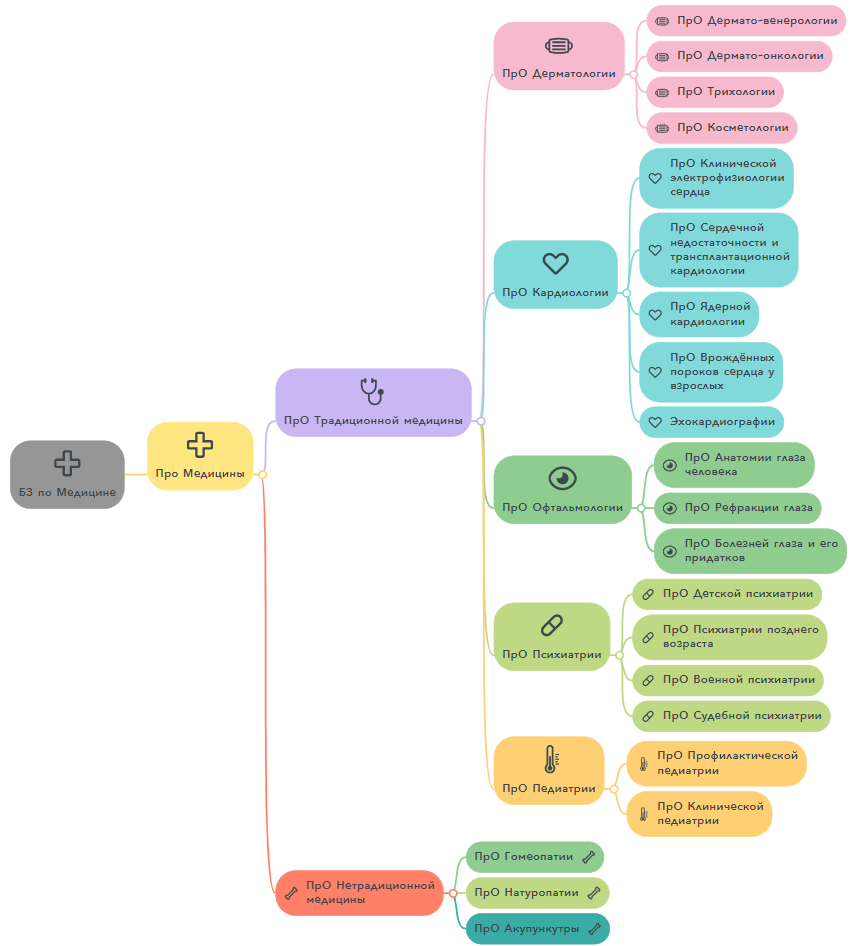
\includegraphics[width=0.95\textwidth]{sections/map.jpeg}
	\caption{Структура БЗ по медицине}
	\label{fig:sections/map}
\end{figure}
Категории пользователей, которыми может быть использована данная система:
\begin{itemize}
	\item Студенты медики;
	\item Преподаватели в медучреждениях;
	\item Медики;
	\item Люди, интересующиеся медициной.
\end{itemize}
\subsection{Характеристика пользователей системы}
Категории пользователей, которыми может быть использована данная система:
\begin{itemize}
	\item Студенты медики;
	\item Преподаватели в медучреждениях;
	\item Медики;
	\item Люди, интересующиеся медициной.
\end{itemize}
Сценарии использования БЗ пользователями отображены на рисунке~\ref{fig:sections/users}.
\begin{figure}[H]
	\centering
	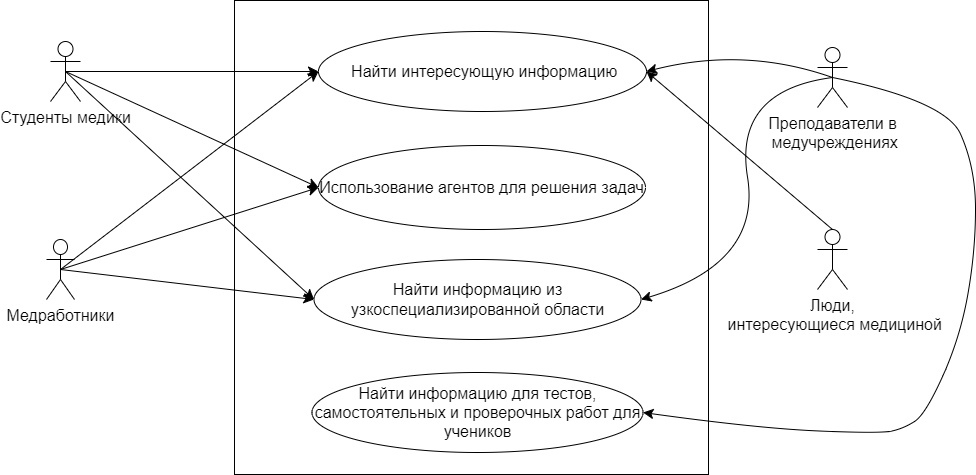
\includegraphics[width=1.0\textwidth]{sections/users.jpeg}
	\caption{Сценарии использования}
	\label{fig:sections/users}
\end{figure}
\subsection{Спецификация предметной области дерматологии}
Про дерматологии включает в себя 4 раздела:
\begin{enumerate}
	\item ПрО дермато-венерологии
	\item ПрО дермато-онкологии
	\item ПрО трихологии 
	\item ПрО косметологии\\
\end{enumerate}

ПрО дерматологии содержит в себе необходимые термины, которые могут быть использованы в других ПрО.
ПрО дерматологии содержит следующие понятия:
\begin{itemize}
	\item дерматология
	\item дерматолог
	\item дерматолог-венеролог
	\item дерматолог-онколог 
	\item дерматолог-трихолог
	\item дерматолог-косметолог
	\item дерматолог-аллерголог
	\item кожные покровы
	\item эпидермис
	\item дерма
	\item гиподерма
	\item волос
	\item роговой слой
	\item базальный слой
	\item сосочковый слой
	\item коллагеновые волокна
	\item сетчатый слой
	\item кератиноциты
	\item сальная железа
	\item глубокая сосудистая сеть
	\item фибробласты
	\item функции кожи
	\item ноготь
	\item матрикс
	\item эпонихий
	\item кутикула
	\item лунка
	\item ногтевая пластина
	\item тело ногтя
	\item боковой валик ногтя
	\item ногтевое ложе
	\item ногтевая пазуха
	\item тело ногтя
	\item свободный край
	\item подногтевая пластина
	\item зуд
	\item шелушение
	\item перхоть
	\item грибковое заболевание кожи
	\item инфекционное заболевание кожи
	\item вирусное заболевание кожи
	\item паразитарное заболевание кожи
	\item воспаление желез
	\item подростковый дерматит
	\item аллергическое высыпание\\
\end{itemize}

\subsection{Спецификация элементов предметной области дерматологии}
Про дерматологии содержит:
\begin{enumerate}
	\item максимальный класс объектов исследования: дерматология
	\item немаксимальный класс объектов исследования: \begin{itemize}
		\item дермато-венеролгия
		\item дермато-онкология
		\item трихология 
		\item дермато-косметология\\
	\end{itemize}
\end{enumerate}
\subsection{Вывод}
В результате проектирования базы знаний по медицине и, в частности,
ПрО дерматологии, была создана эффективная система хранения и управления медицинскими знаниями.

База знаний содержит информацию о строении определённых органов и систем органов человека, различных заболеваниях, перевод всех терминов на латинский язык и английский языки, а также иллюстрации, которые помогают наглядно разобраться в строение органов и систем органов человека.

Важным элементом проектирования базы знаний является возможность ее дальнейшего развития и модификации.

База знаний может быть расширена новыми сведениями о заболеваниях, методах лечения и препаратах, а также может быть адаптирована под различные медицинские специальности.

\section{РЕАЛИЗАЦИЯ БАЗЫ ЗНАНИЙ ПО МЕДИЦИНЕ}
\subsection{Средства, используемые при реализации}
Предметная область медицины реализовывалась на основе технологии OSTIS. Представление знаний в интеллектуальных системах реализуются на основе базового языка – SC-код. С помощью SC-кода можно описывать базы знаний, решатели задач и интерфейс интеллектуальной системы. SC-code является абстрактным языком, но его можно визуализировать в различных формах. 

Формы внешнего представления SC-кода
\begin{itemize}
	\item {SCg (графический)}
	\item {SCs (текстовый линейный)}
	\item {SCn (гипертекстовый)}
\end{itemize}


Для описания понятий использовался подъязык SC-кода - SCs.
SCs-код - линейный вариант представления SC-кода. SCs-код представляет собой множество sc.s-текстов, каждый из которых состоит из sc.s-предложений, разделенных друг от друга двойной точкой с запятой (разделителем sc.s-предложений). При этом sc.s-предложение представляет собой последовательность sc-идентификаторов, являющихся именами описываемых сущностей и разделяемых между собой различными sc.s-разделителями и sc.s-ограничителями. \cite{OSTIS}

Для упрощения процесса разработки исходных текстов баз знаний с использованием SCs-кода вводятся два алфавита символов. Базовый алфавит символов, используемых в sc.s-коннекторах включает только символы, имеющиеся на стандартной современной клавиатуре. Таким образом, для разработки исходных текстов баз знаний, использующих только базовый алфавит символов, используемых в sc.s-коннекторах достаточно обычного текстового редактора. Расширенный алфавит символов, используемых в sc.s-коннекторах включает также дополнительные символы, которые позволяют сделать sc.s-тексты более читабельными и наглядными. Для визуализации и разработки таких sc.s-текстов требуется наличие специальных средств.

Пример формализации понятия с помощью SCs-кода ~\ref{fig:sections/SCs}.
\begin{figure}[H]
	\centering
	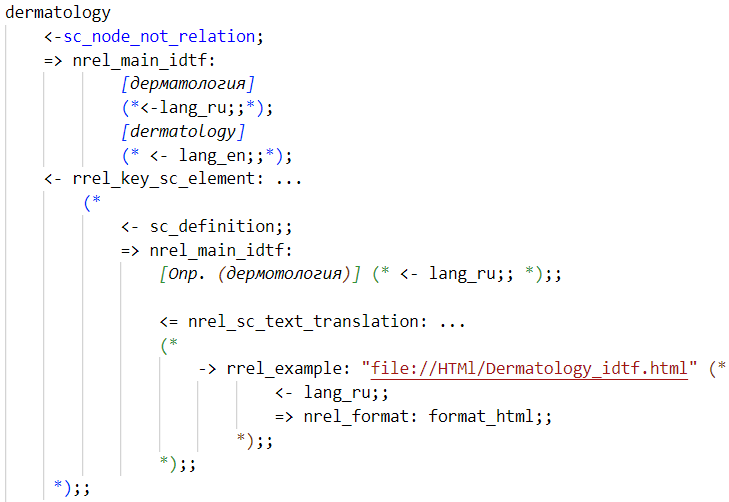
\includegraphics[width=0.7\textwidth]{sections/scs_dermatology.png}
	\caption{SCs-код}
	\label{fig:sections/SCs}
\end{figure}

Пример формализации понятия с помощью языка разметки гипертекста HTML~\ref{fig:sections/HTML}.
\begin{figure}[H]
	\centering
	
\includegraphics[width=0.85\textwidth]{sections/html_hair.png}
	\caption{HTML}
	\label{fig:sections/HTML}
\end{figure}

\subsection{Примеры описания фрагментов базы знаний}
Фрагмент базы знаний, отображающий предметную область дерматологии$,$ представлен на рисунке
~\ref{fig:sections/subject_domain_of_dermatology}.
\begin{figure}[H]
	\centering
	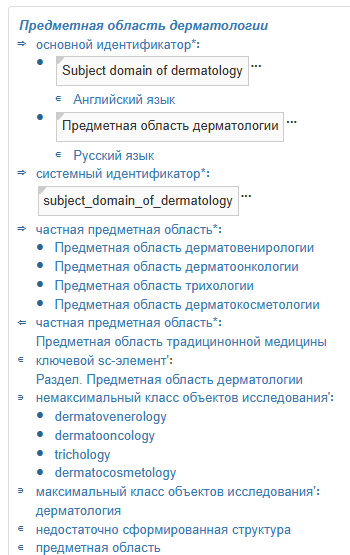
\includegraphics[width=0.7\textwidth]{sections/subject_domain_of_dermatology.png}
	\caption{Предметная область дерматологии}
	\label{fig:sections/subject_domain_of_dermatology}
\end{figure}

Фрагмент базы знаний, отображающий раздел ПрО дерматологии$,$ представлен на рисунке ~\ref{fig:sections/section_of_dermatology}.
\begin{figure}[H]
	\centering
	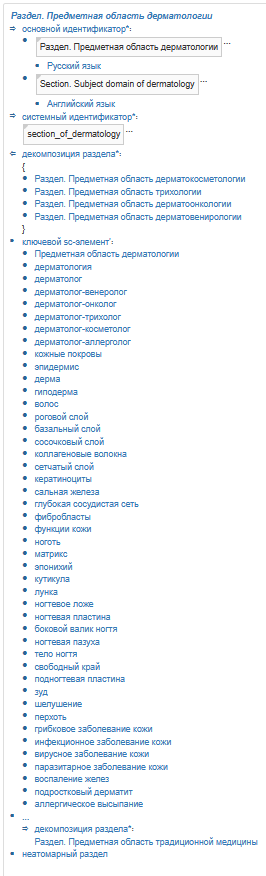
\includegraphics[width=0.4\textwidth]{sections/section_of_dermatology.png}
	\caption{Раздел. Предметная область дерматологии}
	\label{fig:sections/section_of_dermatology}
\end{figure}

Фрагмент базы знаний, отображающий понятие "Дерматология" \cite{bme}$,$ представлен на рисунке
~\ref{fig:sections/concept_dermatology}.
\begin{figure}[H]
	\centering
	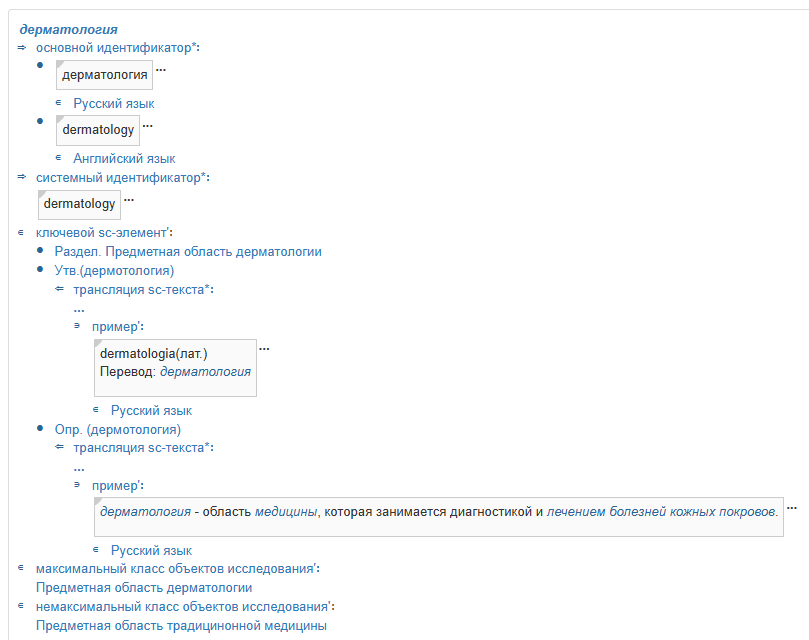
\includegraphics[width=1.0\textwidth]{sections/concept_dermatology.png}
	\caption{Понятие "Дерматология"}
	\label{fig:sections/concept_dermatology}
\end{figure}

Фрагмент базы знаний, отображающий  раздел ПрО дерматоонкологии$,$ представлен на рисунке
~\ref{fig:sections/section_of_dermatooncology}.
\begin{figure}[H]
	\centering
	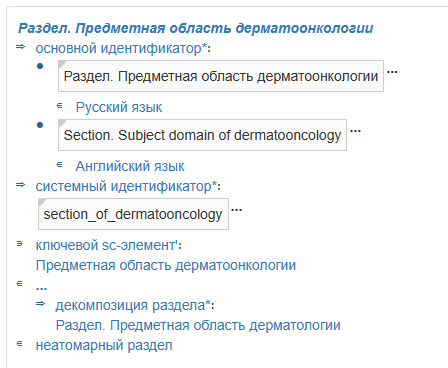
\includegraphics[width=0.5\textwidth]{sections/section_of_dermatooncology.png}
	\caption{Раздел. Предметная область дерматоонколгии}
	\label{fig:sections/section_of_dermatooncology}
\end{figure}
Фрагмент базы знаний, отображающий предметную область дерматоонкологии$,$ представлен на рисунке
~\ref{fig:sections/subject_domain_of_dermatooncology}.
\begin{figure}[H]
	\centering
	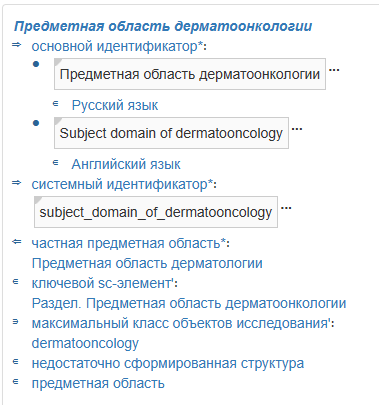
\includegraphics[width=0.65\textwidth]{sections/subject_domain_of_dermatooncology.png}
	\caption{Предметная область дерматонкологии}
	\label{fig:sections/subject_domain_of_dermatooncology}
\end{figure}

Фрагмент базы знаний, отображающий  понятие заболевания "Псориаз" \cite{medi}$,$ представлен на рисунке
~\ref{fig:sections/psoriasis}.
\begin{figure}[H]
	\centering
	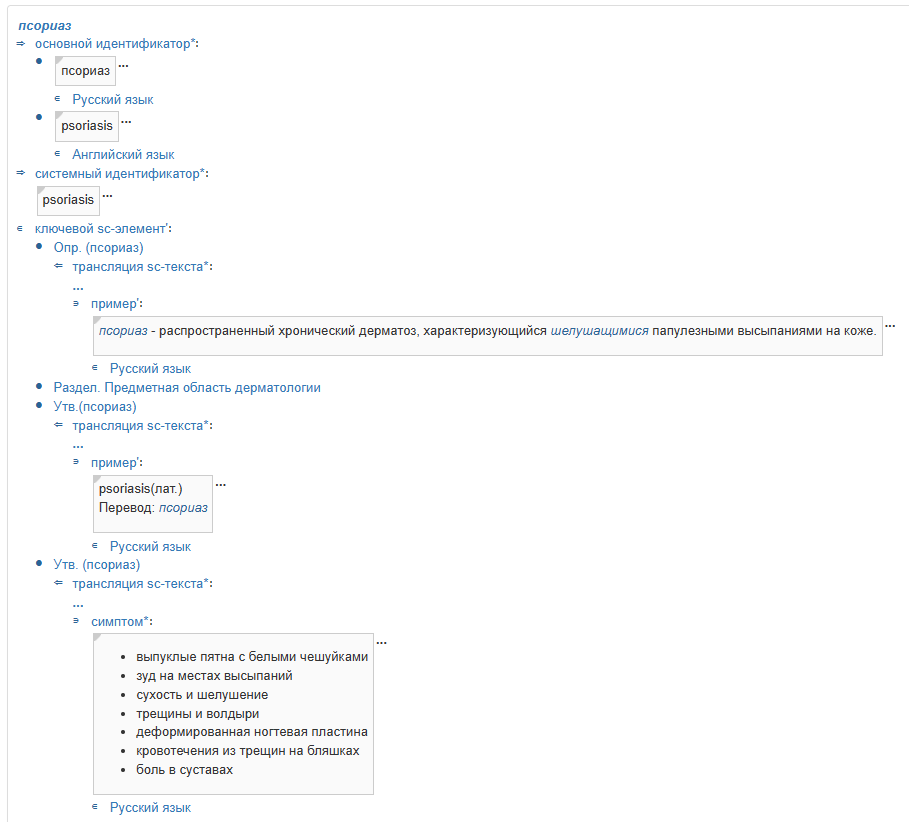
\includegraphics[width=0.95\textwidth]{sections/psoriasis.png}
	\caption{Понятие "Псориаз"}
	\label{fig:sections/psoriasis}
\end{figure}

Фрагмент базы знаний, отображающий  понятие строения органа "Коллагеновые волокна" \cite{bme}$,$ представлен на рисунке
~\ref{fig:sections/concept_collagen_fibers}.
\begin{figure}[H]
	\centering
	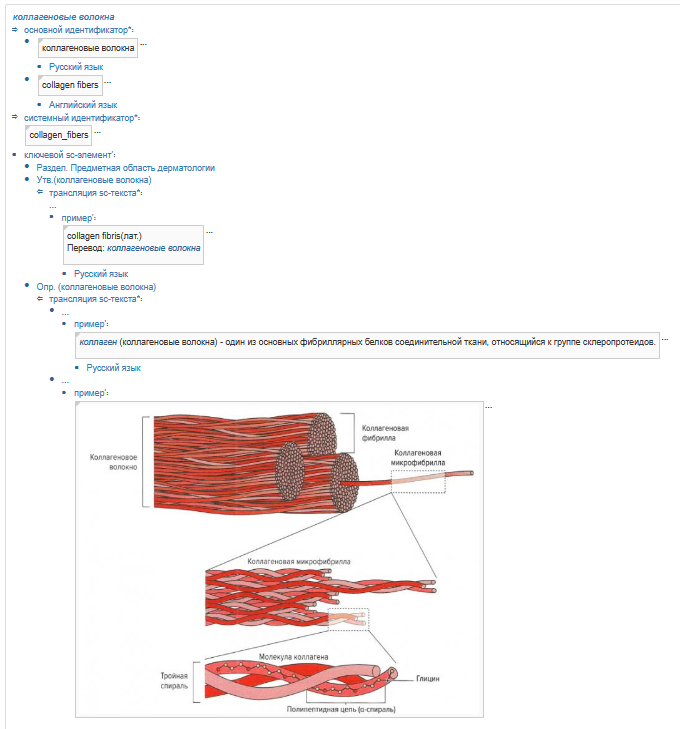
\includegraphics[width=1.05\textwidth]{sections/concept_collagen_fibers.png}
	\caption{Понятие "Коллагеновые волокна"}
	\label{fig:sections/concept_collagen_fibers}
\end{figure}

Фрагмент базы знаний, отображающий  понятие строение органа "Дерма" \cite{bme}$,$ представлен на рисунках
~\ref{fig:sections/derma},~\ref{fig:sections/derma2}
\begin{figure}[H]
	\centering
	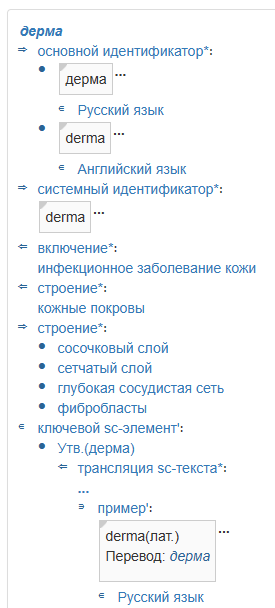
\includegraphics[width=0.45\textwidth]{sections/derma.png}
	\caption{Понятие "Дерма"}
	\label{fig:sections/derma}
\end{figure}
\begin{figure}[H]
	\centering
	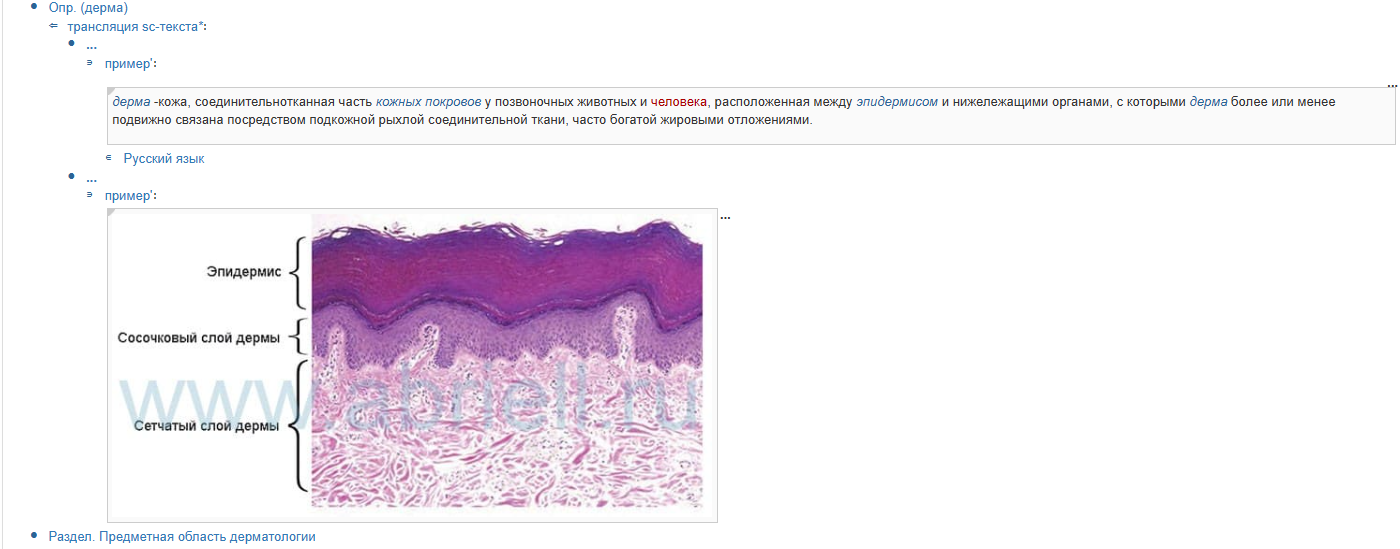
\includegraphics[width=0.95\textwidth]{sections/derma2.png}
	\caption{Понятие "Дерма"}
	\label{fig:sections/derma2}
\end{figure}

Фрагмент базы знаний, отображающий  понятие строение класса заболеваний "Грибковое заболевание кожи" \cite{bme}$,$ представлен на рисунке
~\ref{fig:sections/fungal_infection_of_skin}.
\begin{figure}[H]
	\centering
	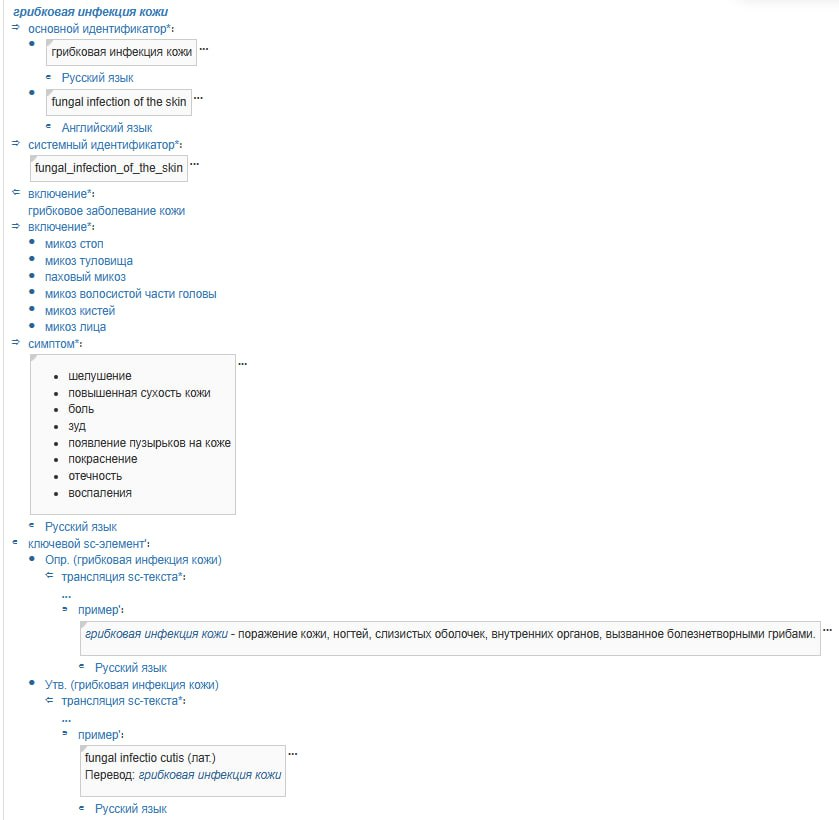
\includegraphics[width=0.95\textwidth]{sections/fungal_infection_of_skin.png}
	\caption{Понятие "Грибковое заболевание кожи"}
	\label{fig:sections/fungal_infection_of_skin}
\end{figure}

\subsection{Тестирование работоспособности базы знаний}
Тестирование базы знаний осуществляется при помощи создания шаблонов для поиска необходимых фрагментов базы знаний.
шаблон для поиска компонентов, составляющих строение эпидермиса
~\ref{fig:sections/pattern_2_der}.
\begin{figure}[H]
	\centering
	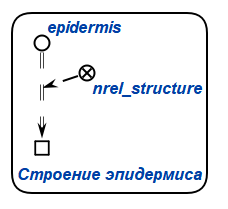
\includegraphics[width=0.5\textwidth]{sections/pattern_2_der.png}
	\caption{Понятие "Шаблон для поиска фрагментов базы знаний"}
	\label{fig:sections/pattern_2_der}
\end{figure}

Результат поиска по шаблону
~\ref{fig:sections/der_2}.
\begin{figure}[H]
	\centering
	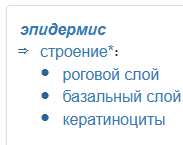
\includegraphics[width=0.5\textwidth]{sections/der_2.png}
	\caption{Понятие "Результат поиска"}
	\label{fig:sections/der_2}
\end{figure}

Шаблон для поиска компонентов, составляющих симптомы всех инфекционных заболеваний кожи
~\ref{fig:sections/pattern_1_der}.
\begin{figure}[H]
	\centering
	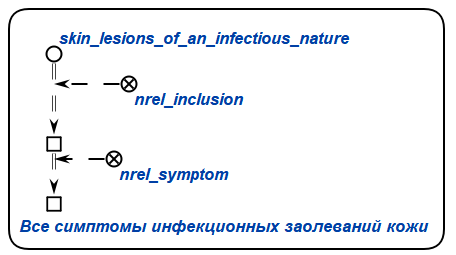
\includegraphics[width=0.8\textwidth]{sections/pattern_1_der.png}
	\caption{Понятие "Шаблон для поиска фрагментов базы знаний"}
	\label{fig:sections/pattern_1_der}
\end{figure}

Результат поиска по шаблону
~\ref{fig:sections/der1_1}, ~\ref{fig:sections/der1_2}.
\begin{figure}[H]
	\centering
	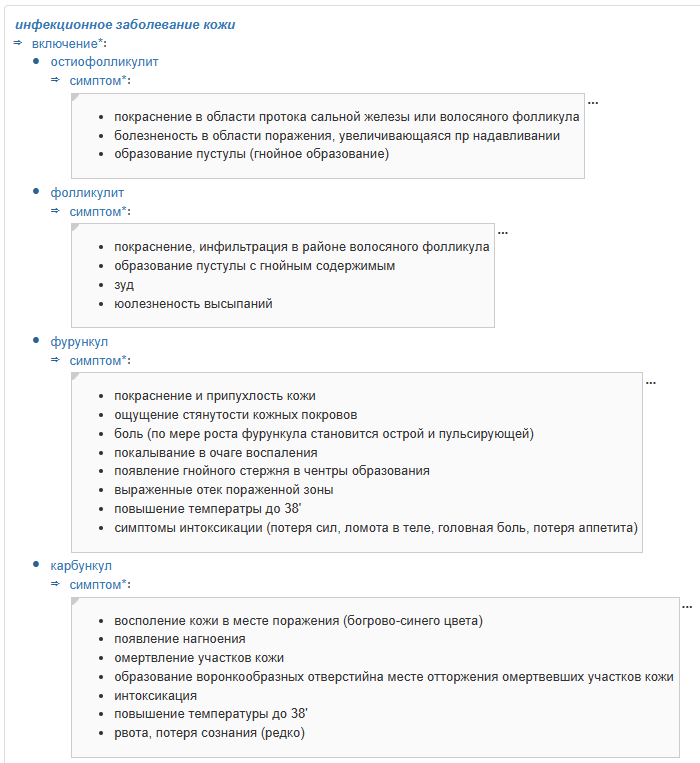
\includegraphics[width=0.8\textwidth]{sections/der1_1.png}
	\caption{Понятие "Результат поиска"}
	\label{fig:sections/der1_1}
\end{figure}

\begin{figure}[H]
	\centering
	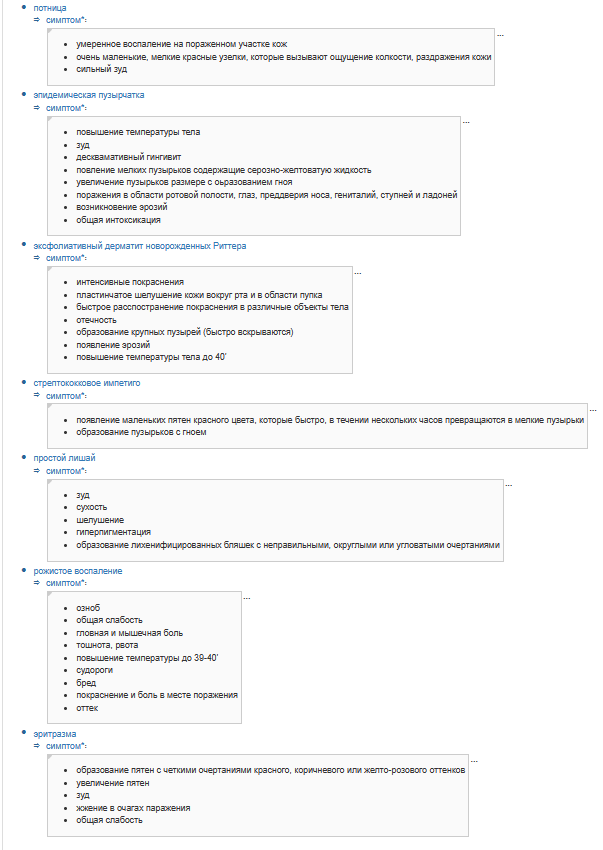
\includegraphics[width=0.7\textwidth]{sections/der1_2.png}
	\caption{Понятие "Результат поиска"}
	\label{fig:sections/der1_2}
\end{figure}

\subsection{Вывод}
В процессе разработки была создана предметная область, не только с большим количество нужной, но и хорошо структурированной информации. Предметные области содержат в себе все необходимые термины, которые имеют перевод на латинский язык. Также, многие термины имеют графический вид представления (иллюстрации), симптомы заболевания, и строение органов и систем органов. Структура данной информации очень удобна для восприятия пользователями, что значительно облегчит поиск всей необходимо информации. 

\sectioncentered*{ЗАКЛЮЧЕНИЕ}
\addcontentsline{toc}{section}{ЗАКЛЮЧЕНИЕ}

В рамках курсовой работы была разработана база знаний интеллектуальной справочной системы по медицине, включающая в себя раздел медицины,который декомпозируется на два основных раздела: традиционной и нетрадиционной медицины. Раздел нетрадиционной медицины состоит из 3 подразделов: гомеопатии, натуропатии, акупунктуры.  Раздел традиционной медицины состоит из 5 подразделов: дерматологии, психиатрии, педиатрии, офтальмологии, кардиологии. Данные разделы также делятся на свои специфические подразделы. Разрабатываемая мной, предметная область дерматологии содержит подразделы: дермато-венерологии, дермато-онкологии, трихологии и косметологии.

Суммарно в предметной области дерматологии было формализовано более 50 абсолютных понятий. Понятия представляются на 3 языках, содержат описание, в которых есть гиперссылки на другие понятия связанные с ним. Также, иллюстрации, которые помогают лучше усваивать информацию, а заболевания и патологии содержат в себе симптоматику.

Для реализации данной базы знаний использовалась технология OSTIS. Поскольку база знаний, построенная по технологии OSTIS, может описывать любой вид знаний, удобна как для машинной обработки, так и восприятия человеком. 

В результате было положено начало созданию базы знаний интеллектуальной справочной системы по медицине.

Данная система сможет помочь студентам-медикам, медработникам и простым пользователям, интересующимся медициной, облегчить обучение и сэкономить время на поиски нужной информации. Система хорошо структурирована и наполнена большим количеством необходимой информации, что исключает необходимость использования большого количества разных источников по интересующему вопросу.

Также данная система может помочь преподавателям в медучреждениях быстро и легко находить информацию для различных проверочных  и контрольных работ для студентов. 

В дальнейшем планируется пополнение базы знаний новыми понятиями и модернизация старых. Так как в медицине существует огромное множество разделов и охватить их в рамках только лишь одной курсовой работы невозможно.
